\section{API documentation}
\label{secD4:APIDocumentation}
Le API fornite dall’applicazione PlanIt e già descritte nella sezione precedente \ref{apd:SviluppoAPI} sono
state documentate utilizzando il modulo di NextJS chiamato "next-swagger-doc". In questo
modo la documentazione relativa alle API è direttamente disponibile a chiunque veda il codice
sorgente.\\
Per poter generare l’endpoint dedicato alla presentazione delle API abbiamo utilizzato "swagger-ui-react" in quanto crea una pagina web secondo la documentazione scritta.
In particolare, di seguito mostriamo la pagina web relativa alla documentazione che presenta le 12 API, di cui ce ne sono sia di tipo GET che POST che DELETE, essenziali per la gestione del prototipo del sito PlanIt che è stato sviluppato.\\
Nella pagina della documentazione fornita, abbiamo reso disponibile anche la possibilità di utilizzare degli esempi preparati "ad hoc" per poter vedere come funzionano tutte le API da noi implementate. \\
L’endpoint da invocare per raggiungere la seguente documentazione e’:
\href{http://localhost:3000/ApiDoc}{http://localhost:3000/ApiDoc} oppure \href{http://127.0.0.1:3000/ApiDoc}{http://127.0.0.1:3000/ApiDoc}
Inoltre, la documentazione è possibile visionarla non solo, grazie al codice sorgente da noi sviluppato, ma anche direttamente al seguente link dove abbiamo effettuato l'hosting della documentazione: \href{https://plan-it.it/apidoc}{https://plan-it.it/apidoc}. Infatti abbiamo usato il sito "netlify" per l'hosting di ciò che abbiamo implementato per questo deliverable D4, in modo tale che la documentazione e anche il FrontEnd, il cui link verrà passato successivamente, possano essere sempre raggiungibili anche senza dover avere per forza il codice sorgente da eseguire.
\begin{center}
    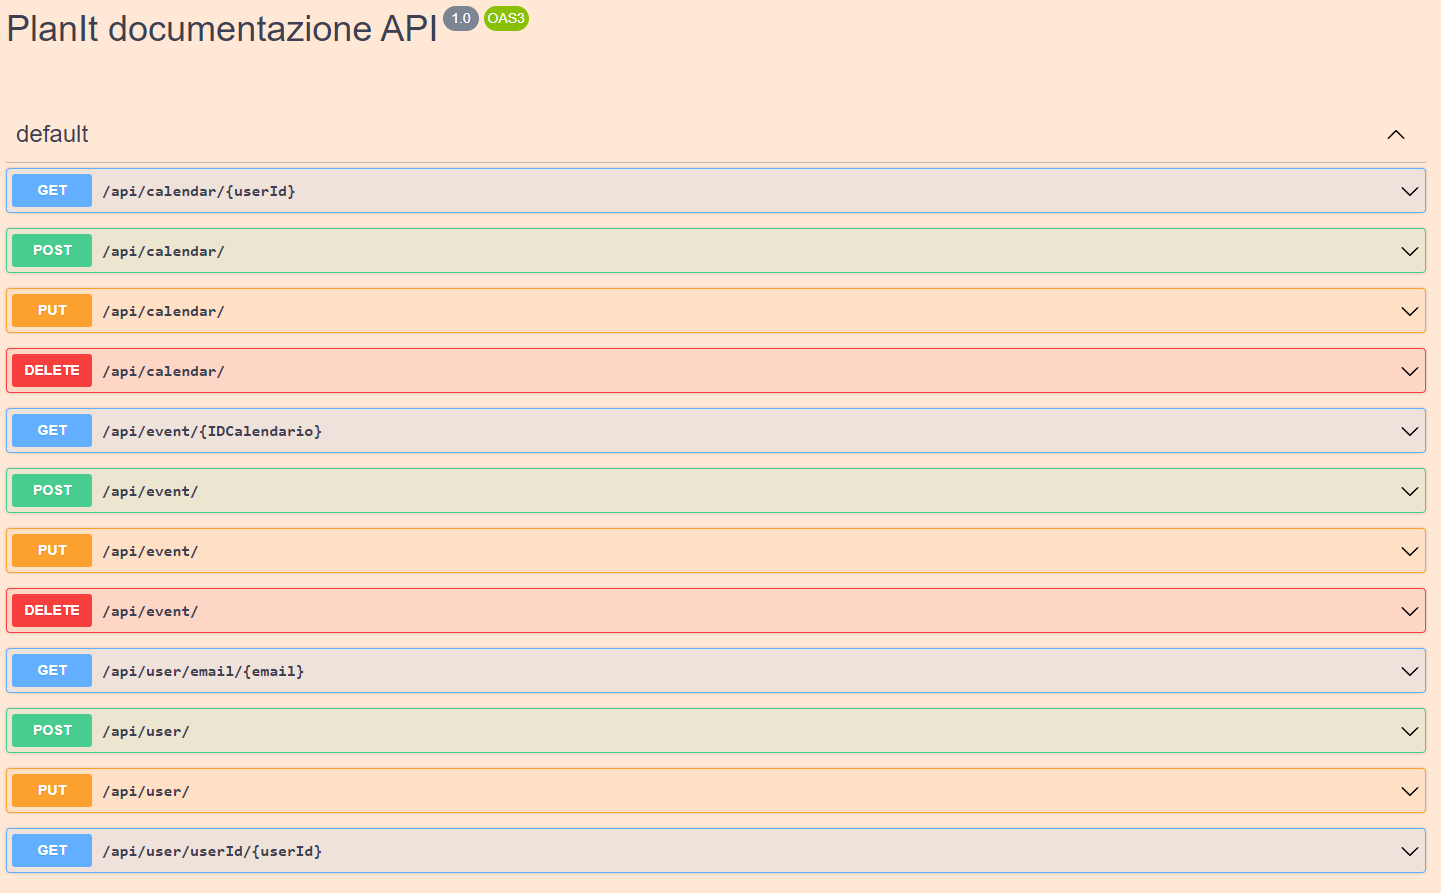
\includegraphics[width=1\textwidth, height=0.4\textheight]{img/png/documentazione.png}
    \captionof{figure}{Documentazione}
    \blfootnote{Immagine \href{https://github.com/Life-planner/Documentazione/blob/main/D4/img/png/documentazione.png}{PNG} Documentazione}
\end{center}